\appendix
\chapter{Anlagen}
\section{Well-Known-Binary Format (WKB)}
\label{sec:appendix:wkb}
Das \textit{Well-Known-Binary} Format ist die binäre Repräsentation eines geometrischen Objekts des \textit{Simple Feature Models}.
Das Simple Feature Model ist eine Untermenge des ISO 19107 Standards, welcher die geometrischen Eigenschaften von Geoobjekten spezifiziert. Ausgehend von einer allgemeinen Oberklasse können geometrische Primitive, wie z.B. ein Punkt, oder komplexe geometrische Objekte, wie z.B. Flächen oder Sammlungen von Objekten, beschrieben werden. (vgl. \cite{Bill2010}:358ff.). Die verfügbaren Klassen werden in Abbildung \ref{fig:bill_sfm} aufgezeigt.
\begin{figure}[!htb]
  \centering
   \fbox{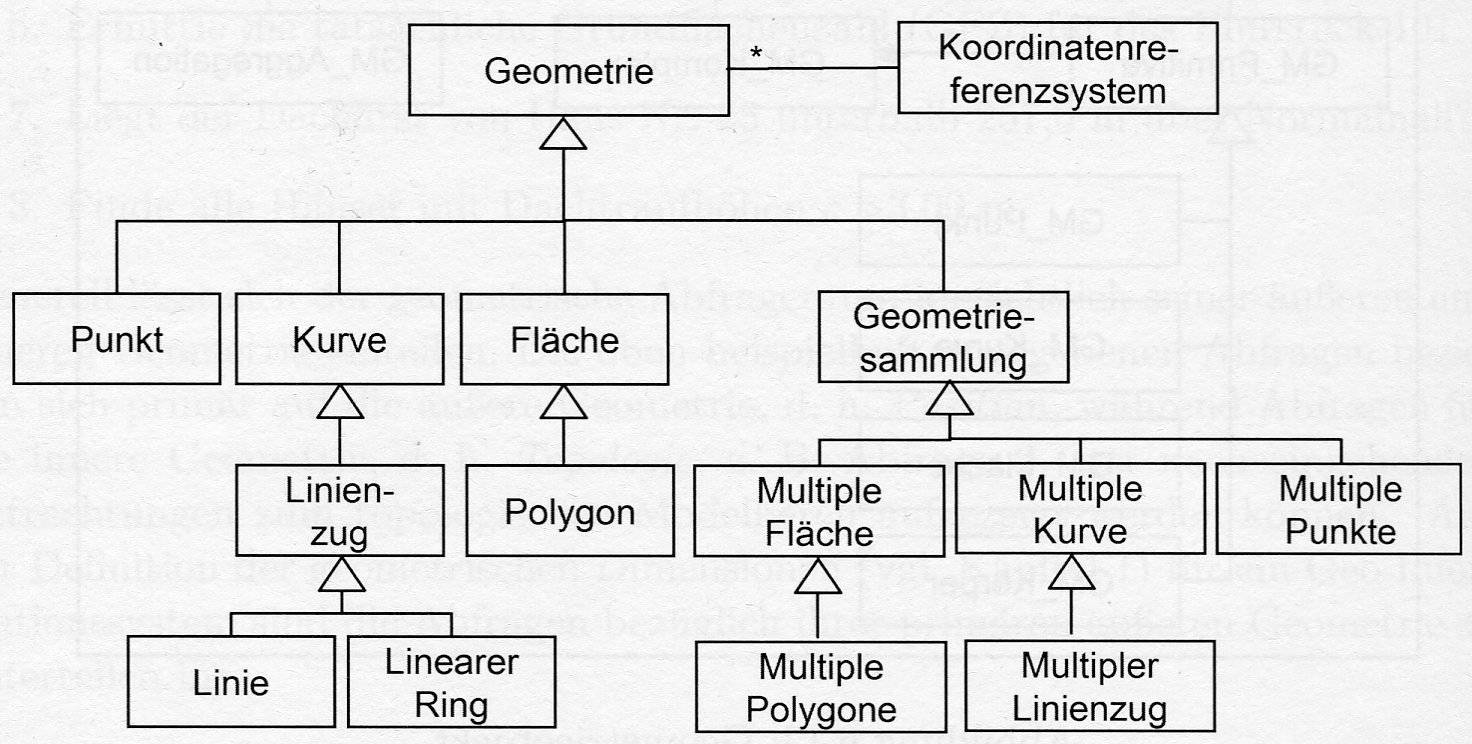
\includegraphics[width=1\textwidth]{gfx/bill_sfm001.jpg}}
   \caption{Geometrien im Simple Feature Model \protect\cite{Bill2010}:360}
   \label{fig:bill_sfm}
\end{figure}

Das WKB Format wird beispielsweise innerhalb der PostgreSQL Erweiterung PostGIS\footnote{http://postgis.net} genutzt, um geometrische Objekte in einer Datenbank abzulegen.
Analog dazu existiert das \textit{Well-Known-Text} Format, welches die textuelle Repräsentation geometrische Objekte des Simple Feature Models spezifiziert.

\subsubsection{Beispiel für das WKB und das WKT Format}
Ein Punkt mit den Koordinaten \texttt{13.439561 Ost} sowie \texttt{52.54002 Nord} entspricht der WKT Repräsentation\\\\
\texttt{SRID=4326;POINT(13.439561 52.54002)}\\\\
und der WKB Repräsentation\\\\
\texttt{0101000020E6100000B131AF230EE12A40CC9717601F454A40}\\\\
Der Wert \texttt{SRID} beinhaltet die ID des zu verwendenden Koordinatenreferenzsystems.
Die ID \texttt{4326} entspricht dem häufig verwendeten Referenzsystem \texttt{WGS84}\footnote{http://spatialreference.org/ref/epsg/4326/}.  

\section{GeoJSON}
\label{sec:appendix:geojson}
GeoJSON\footnote{http://geojson.org} ist ein Format zur Repräsentation von geometrischen Objekten im JSON Format.
Es verwendet ein ähnliches hierarchisches Klassenmodell. (vgl. \cite{WEB:GEOJSON:Spec:2008}).

\subsubsection{Beispiel für das GeoJSON Format}
Ein Punkt mit den Koordinaten \texttt{13.439561 Ost} sowie \texttt{52.54002 Nord} entspricht der GeoJSON Repräsentation
\begin{lstlisting}
  {
    "type": "Point",
    "coordinates": [
        13.439561,
        52.54002
    ]
}
\end{lstlisting}

\section{OpenStreetMap Datenformat}
\label{sec:appendix:osm:data}

\section{Beispiel einer Straße in OpenStreetMap}
\label{sec:appenix:osm:streets}